\section{Common (Networking)}\label{sec:common}

This library handles the communication between the \code{Client} and the
\code{Server}. The \code{RequestMessage} class represents a request made by the
client, while the \code{ResponseMessage} class represents a response from the
server. Both classes contain a list of entities (Java classes) that contains the
data. The \code{RequestMessage} class also contains the auth token used for
authenticating the user.

The library serialize all messages in XML\@.

\begin{landscape}
	\begin{figure}[!ht]
		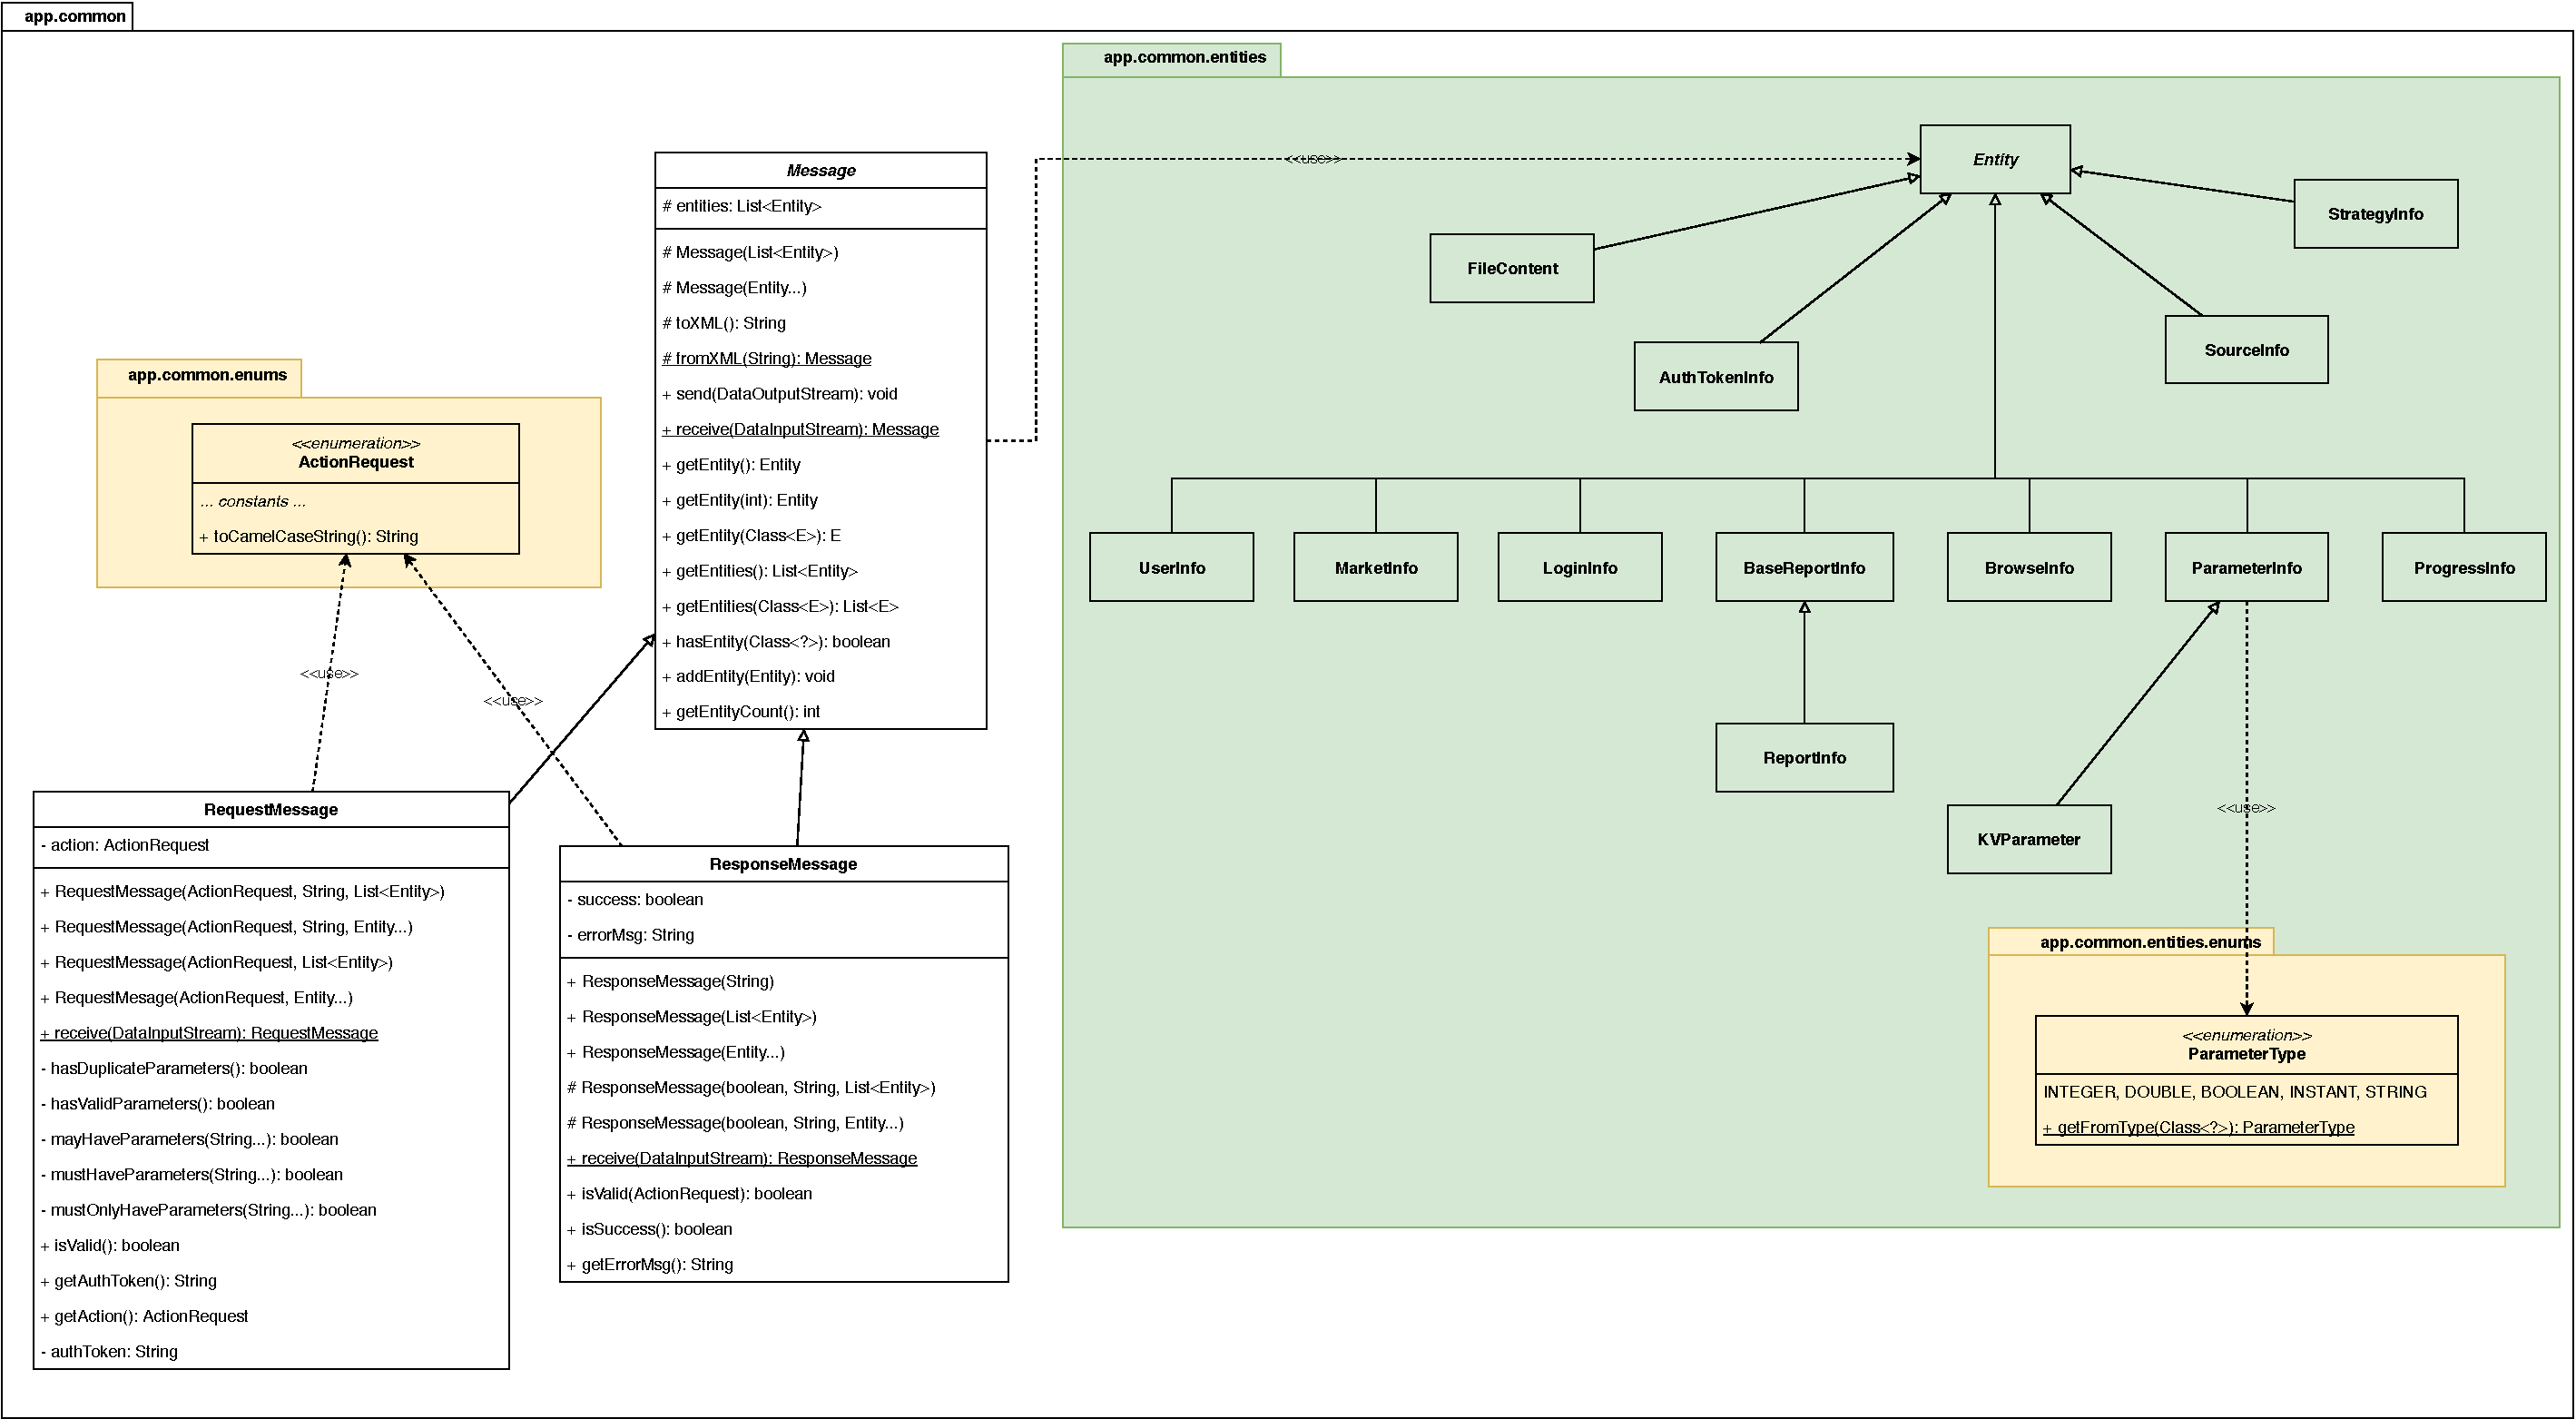
\includegraphics[width=0.8\paperheight]{module-common}
		\caption*{\textbf{Figure~\ref{fig:common}}}
		\captionlistentry{}\label{fig:common}
	\end{figure}
\end{landscape}
